\chapter{Capacidad de las métricas}\label{sec:diferencias}
\addcontentsline{toc}{chapter}{Capacidad de las métricas}

En este capítulo se muestran una serie de estudios estadísticas que muestran la capacidad de todas y cada una de las métricas para diferenciar entre los grupos de prácticas en riesgo y los que no tienen problemas para resolver los problemas propuestos por el profesor.

\subsection{Estudio de la capacidad de separación de las medidas clásicas del rendimiento}

\subsection{Estudio de la capacidad de separación de las medidas de complejidad de propósito general}

\begin{figure}[H]
\centering
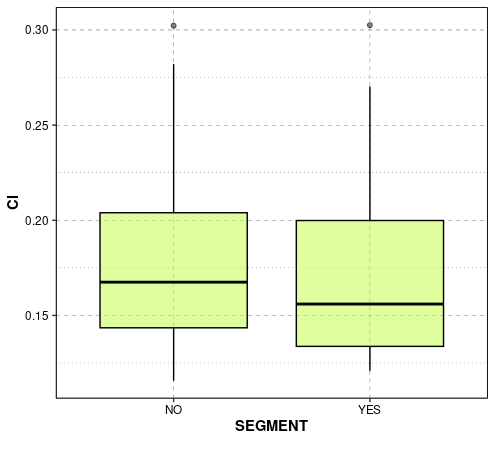
\includegraphics[width=0.3\textwidth]{diferencias/cl.png}
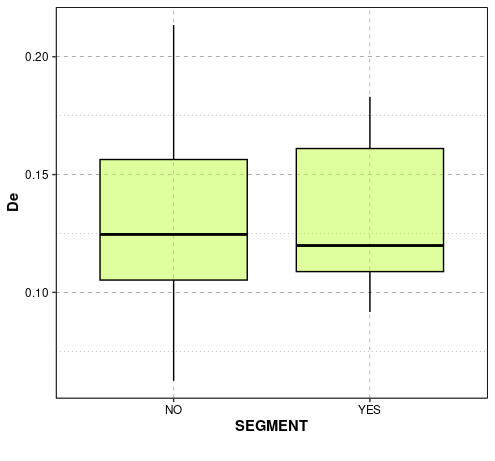
\includegraphics[width=0.3\textwidth]{diferencias/de.png}
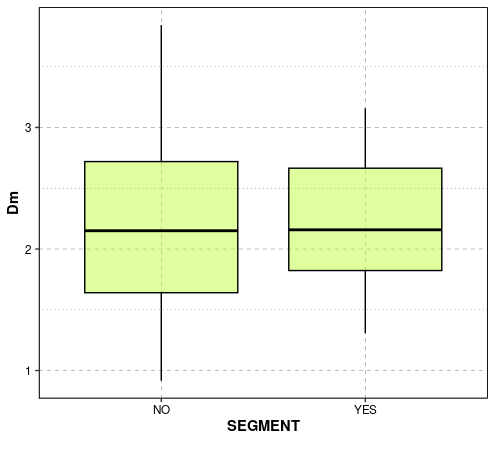
\includegraphics[width=0.3\textwidth]{diferencias/dm.png} \\
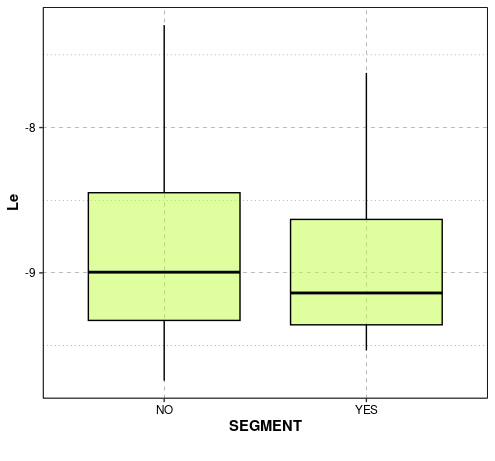
\includegraphics[width=0.3\textwidth]{diferencias/le.png}
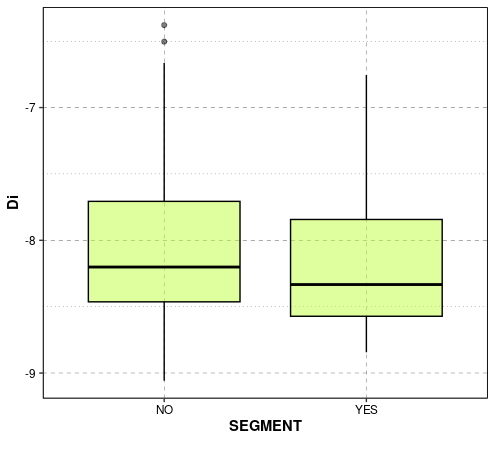
\includegraphics[width=0.3\textwidth]{diferencias/di.png}
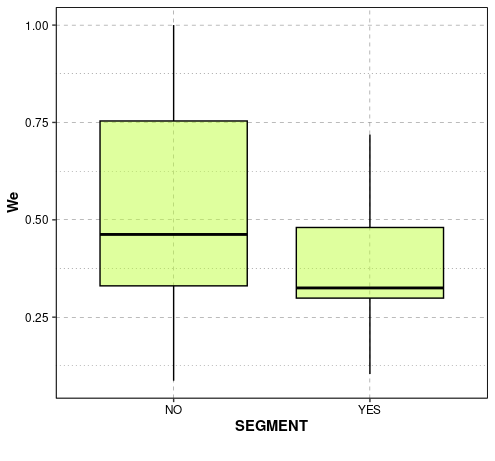
\includegraphics[width=0.3\textwidth]{diferencias/we.png} \\
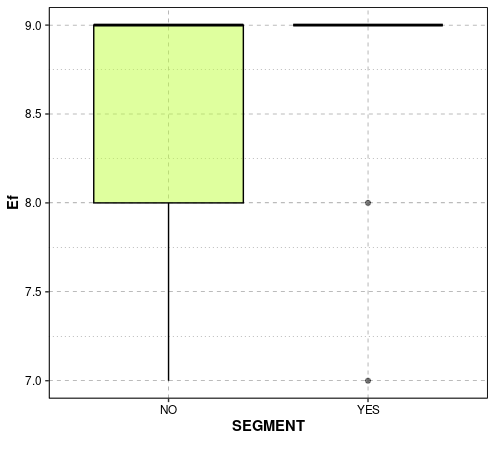
\includegraphics[width=0.3\textwidth]{diferencias/ef.png}
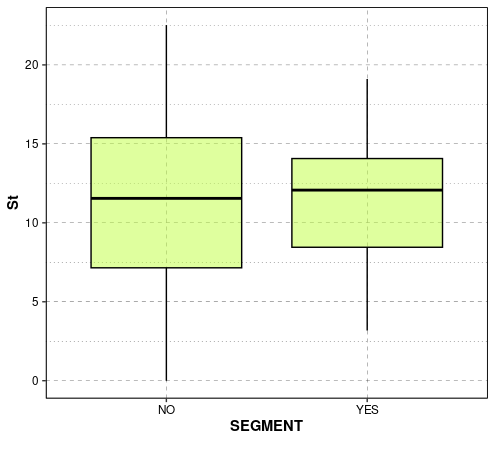
\includegraphics[width=0.3\textwidth]{diferencias/st.png}
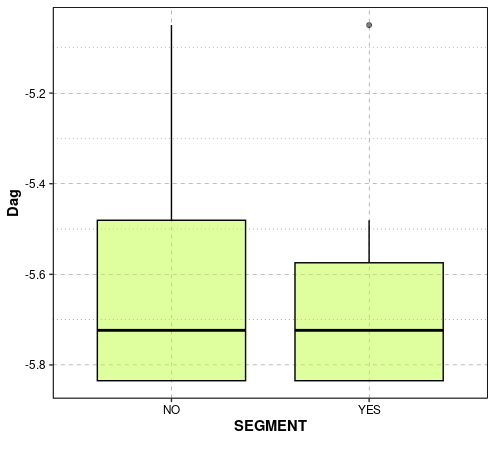
\includegraphics[width=0.3\textwidth]{diferencias/dag.png} \\
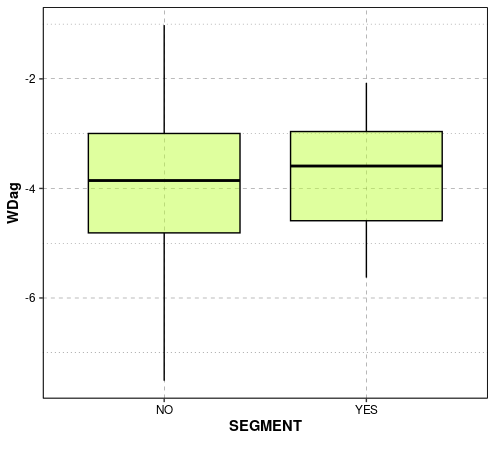
\includegraphics[width=0.3\textwidth]{diferencias/wdag.png}
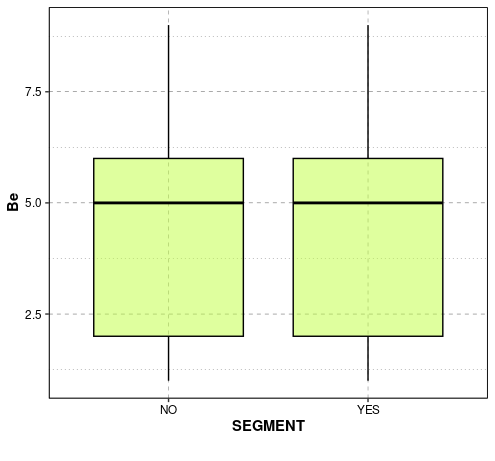
\includegraphics[width=0.3\textwidth]{diferencias/be.png}
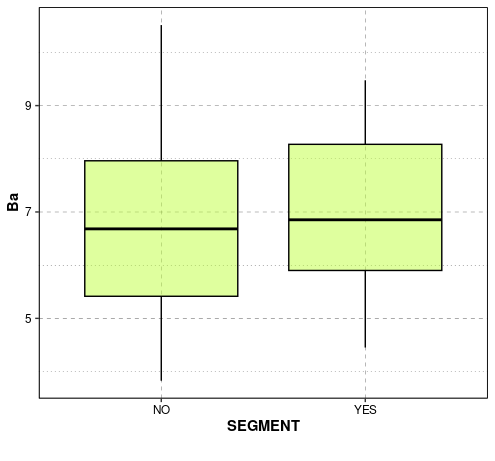
\includegraphics[width=0.3\textwidth]{diferencias/ba.png}
\caption{Boxplots de las diferentes medidas de complejidad por grupos de alumnos.}
\label{fig:tstudentcomplexity}
\end{figure}

\begin{figure}[H]
\centering
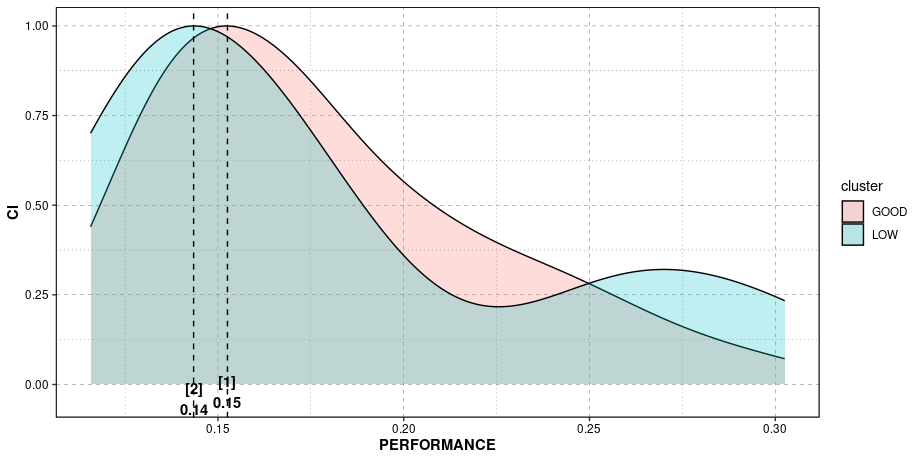
\includegraphics[width=0.48\textwidth]{diferencias/densitycl.png}
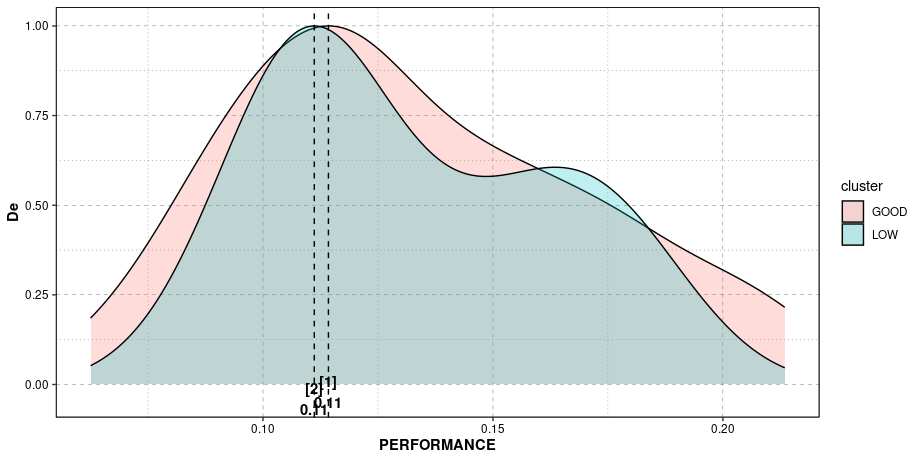
\includegraphics[width=0.48\textwidth]{diferencias/densityde.png} \\
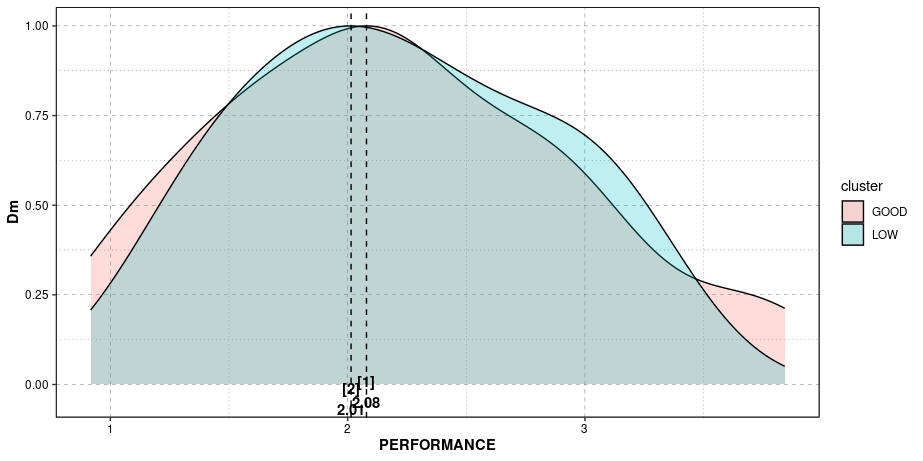
\includegraphics[width=0.48\textwidth]{diferencias/densitydm.png}
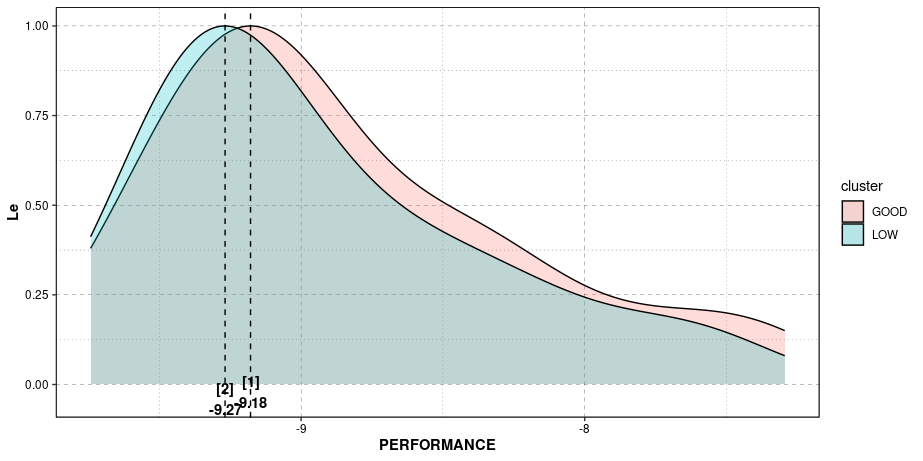
\includegraphics[width=0.48\textwidth]{diferencias/densityle.png} \\
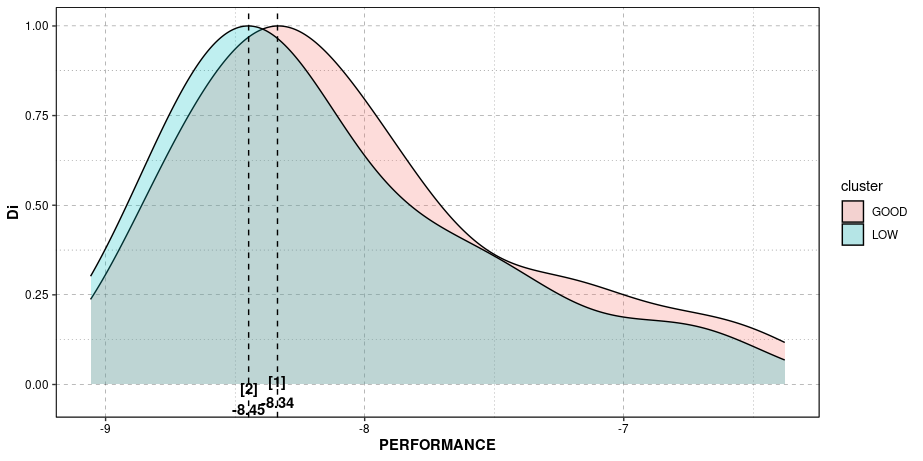
\includegraphics[width=0.48\textwidth]{diferencias/densitydi.png}
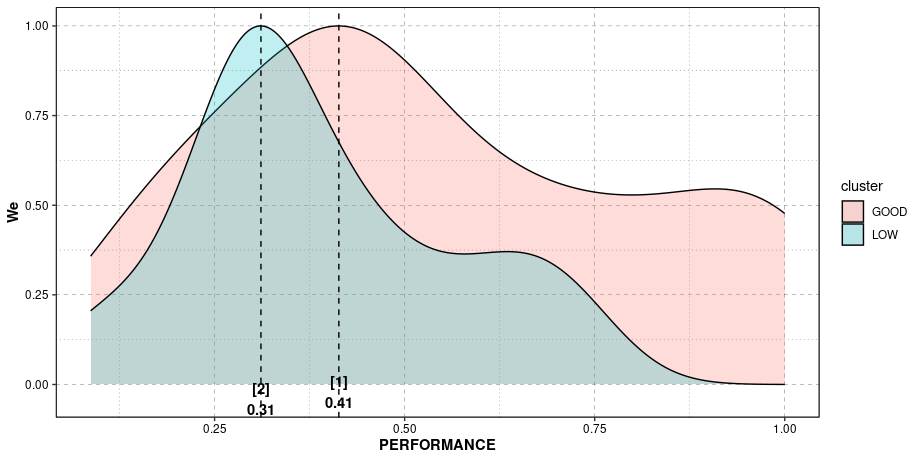
\includegraphics[width=0.48\textwidth]{diferencias/densitywe.png} \\
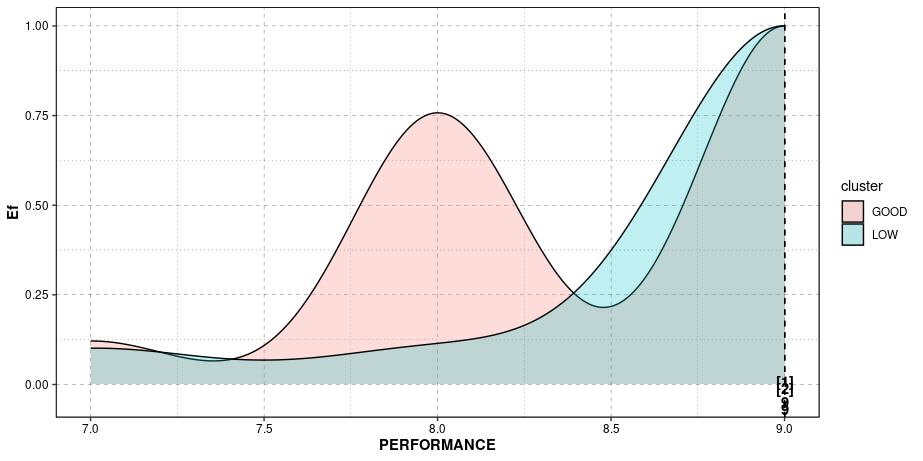
\includegraphics[width=0.48\textwidth]{diferencias/densityef.png}
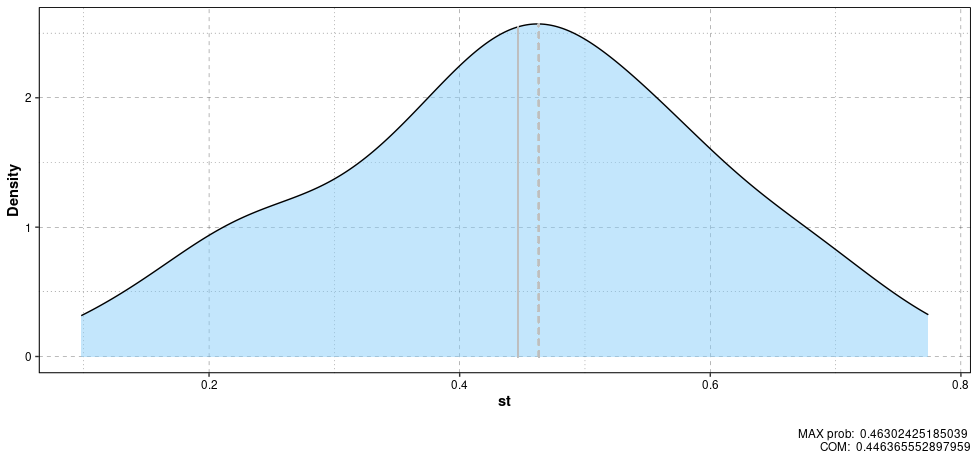
\includegraphics[width=0.48\textwidth]{diferencias/densityst.png} \\
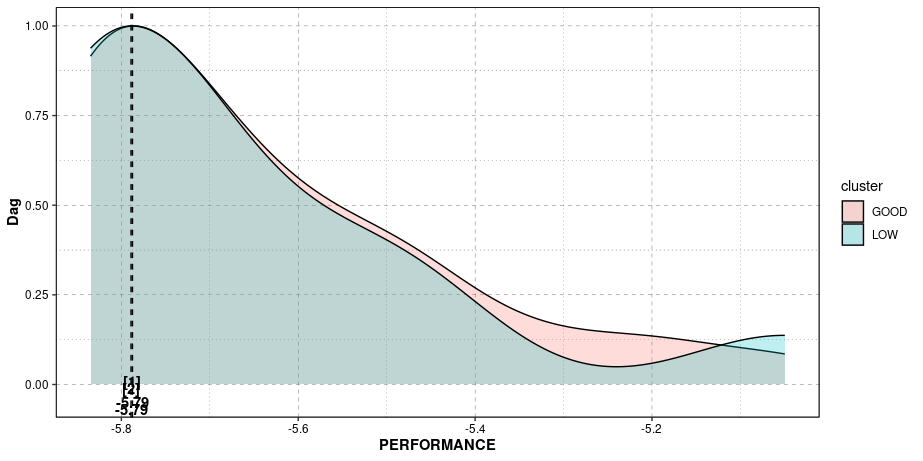
\includegraphics[width=0.48\textwidth]{diferencias/densitydag.png}
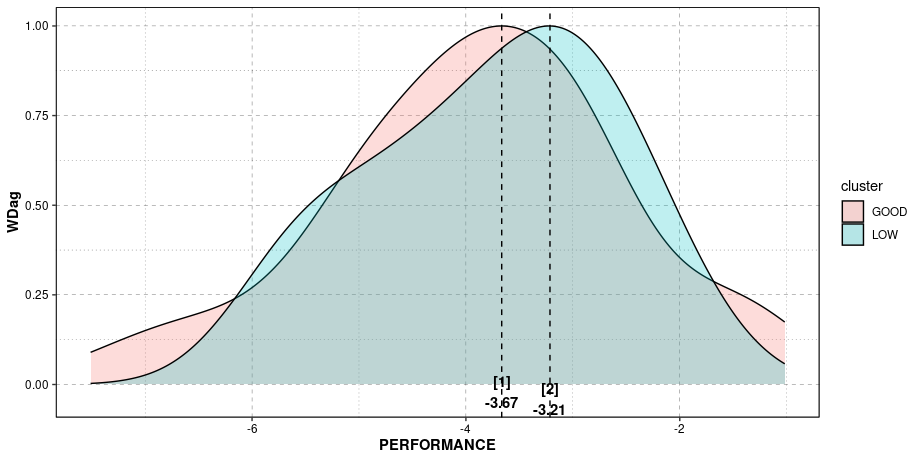
\includegraphics[width=0.48\textwidth]{diferencias/densitywdag.png} \\
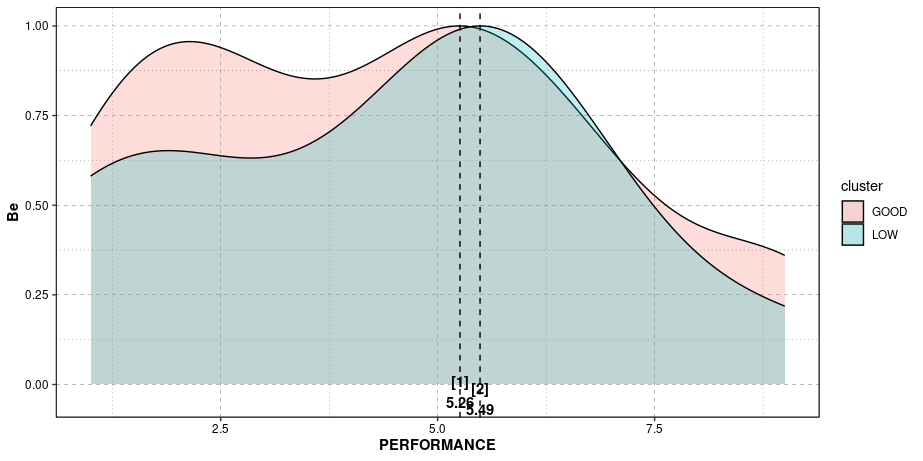
\includegraphics[width=0.48\textwidth]{diferencias/densitybe.png}
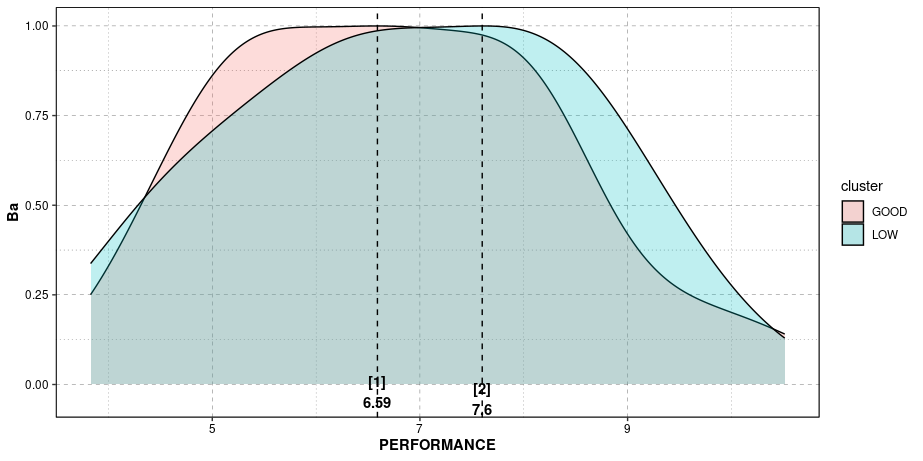
\includegraphics[width=0.48\textwidth]{diferencias/densityba.png}
\caption{Funciones de densidad de las diferentes medidas de complejidad por grupos de alumnos.}
\label{fig:tstudentcomplexitydensity}
\end{figure}

